%!TEX root = main.tex

\section{Implementation} % (fold)
\label{sec:implementation}

\subsection{Client} % (fold)
\label{sub:client}
Client accepts user's input. It's a lazy interactive console.
User would define their RDD lineage. But until any action is called, there is no real computation at all.
It will record down the parent RDD and the function or other parameters related to the RDDs\@.
If it's a wide dependency, it will first create a Repartition RDD between itself and its parent.

When user called a action, Client will firstly create the Partition lineage based on the given RDD lineage as Figure~\ref{fig:partition_lineage}.
Any Partition will only have the dependency links to the partitions it needs in the parent RDD\@.
If it's a narrow dependency, it will only have one dependency partition.
And if it's a wide dependency, it will depend on multiple ones.
By limiting the reference inside Partition object,
it becomes easy to dump the partition object by CloudPickle\cite{cloudpickle} without introduce any unnecessary object,
which will reduce data transferring and dump failure.

Secondly, for every partition in the final target RDD, the client will create a job for it.
And broadcast them by partitions' uuid.
Only these partitions will be created as a job,
because these partitions are the ones that the user really care about, not those intermediate results.

Finally, it will keep discovering for the finished Partitions of these jobs.
And fetch them back to local when find them available in the cluster.
Merge the results of those partitions and return final result to the user.
% subsection client (end)

\begin{figure}[htb]
    \centering
    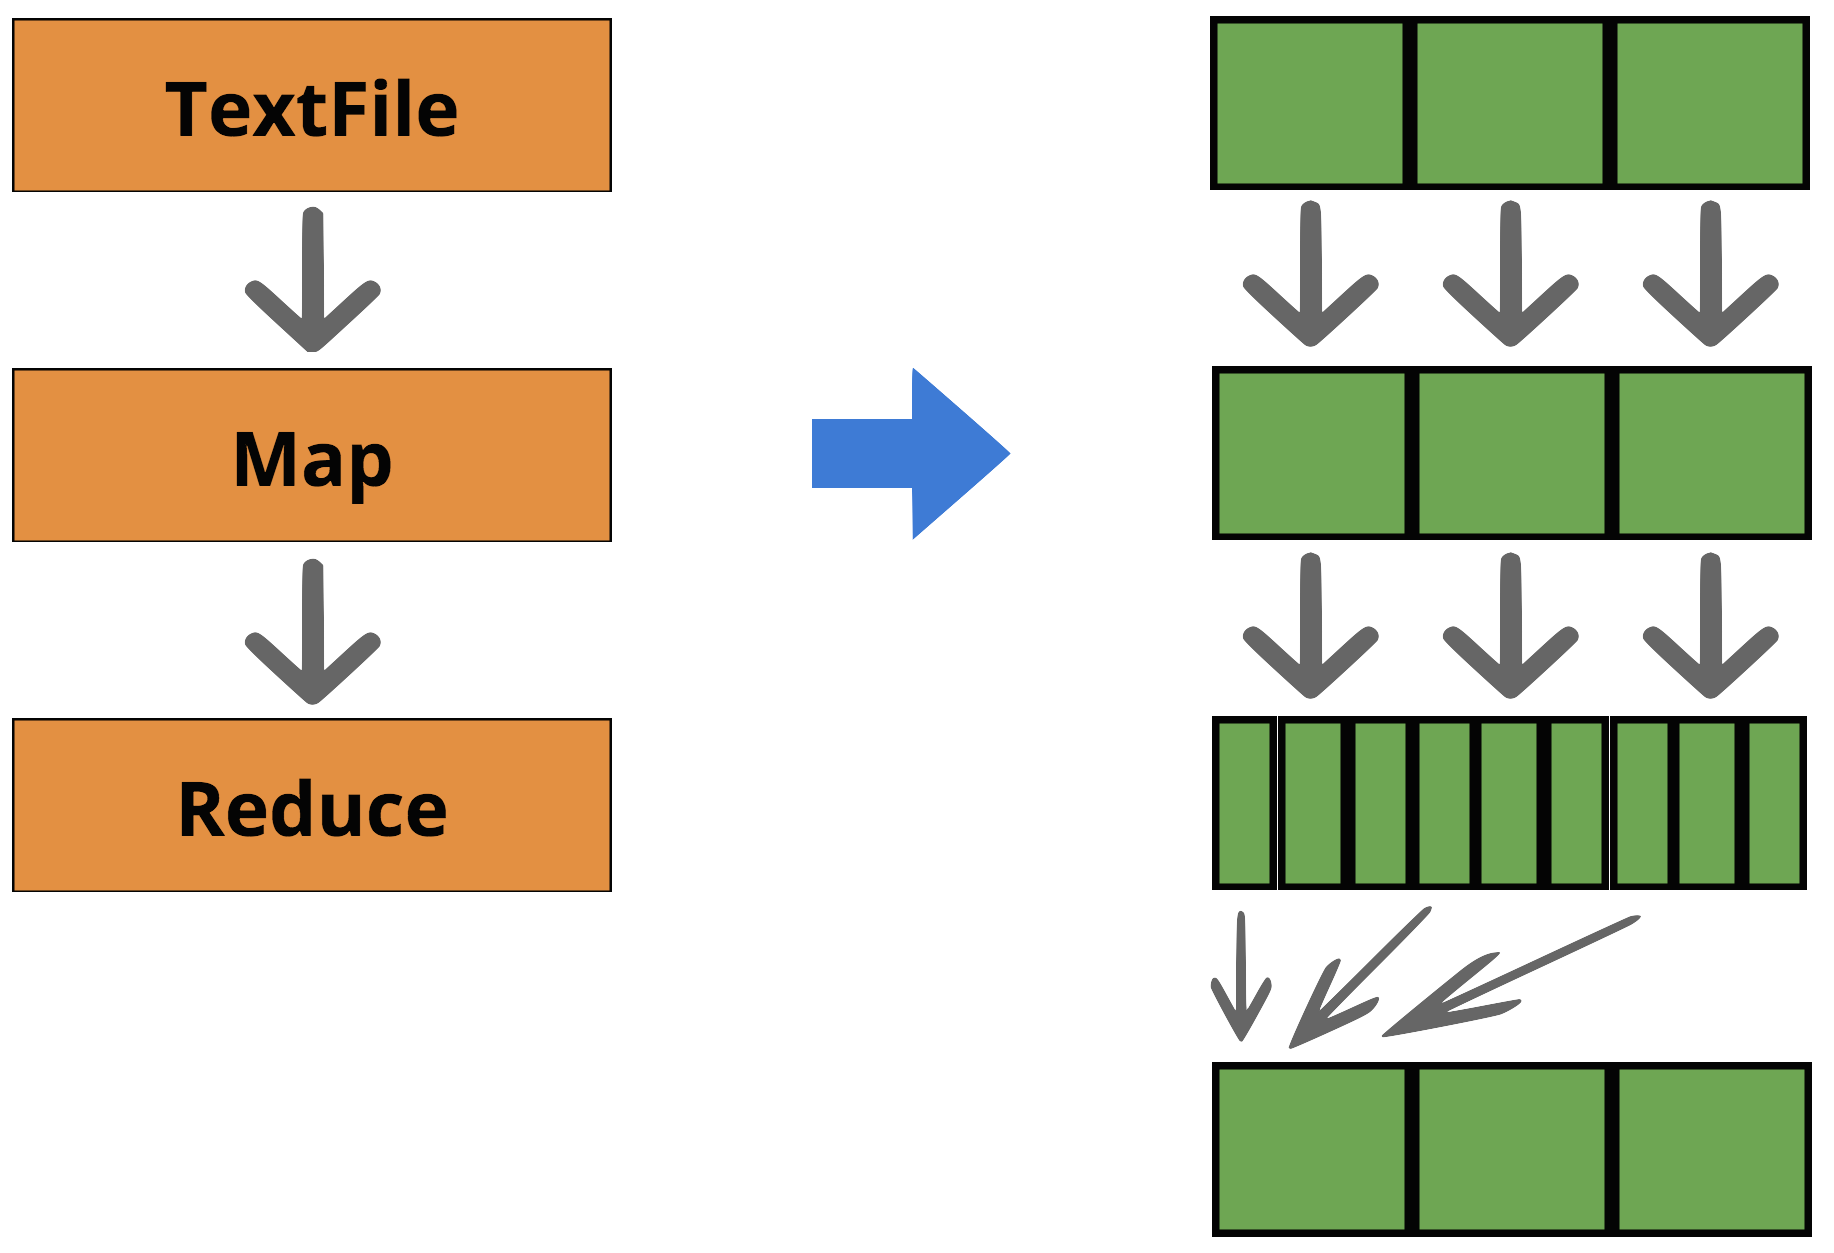
\includegraphics[width=0.4\textwidth]{images/partition_lineage.png}
    \caption{RDD Lineage to Partition Lineage}\label{fig:partition_lineage}
\end{figure}

\subsection{Worker} % (fold)
\label{sub:worker}
When the Job Discoverer of a Worker finds a job broadcasted in the cluster,
it will connect back to the source and retrieve the corresponding Partition object back,
and add it to the Worker's Jobs queue.

Worker has a thread that keep trying to take the Partition object out of the Jobs queue.
After successfully taken one out, it will call the Partition object's function.
For the narrow dependency transform, like Map and Filter, it will directly call the parent partition's function.
For the wide dependency transform, like Repartition, more works will be done.

First, it will check all the dependency partitions in its own Partition Discoverer,
and save the results to the Partition objects.
If that partition is local, the discoverer will simply return the partition's result.
Otherwise, it will connect to the remote worker, fetch the result back, and cache it locally for the future needs.

Second, the worker will find all the missing parent partitions that can't be found in the cluster.
If any parent partition is missing, it will wrap them as a Job and broadcast it.
Then suspend the current job by appending it to the end of the jobs queue.
If all parent partitions are done, the worker will compute the current job, since all the dependencies are local now.
And put it into Partition Broadcaster to announce that the partition is finished in the cluster.
% subsection worker (end)

\subsection{Broadcaster} % (fold)
\label{sub:broadcaster}
Broadcast system is based on UDP broadcast.
One side of broadcasters and discoverers will keep sending packages starts with a magic prefix string,
to a predefined multi-cast address.
The other side will keep receiving packages from that address and filter packages with the magic prefix string.

A python wrapper called MinusConf\cite{minusconf} is used with gevent\cite{gevent} monkey-patching.
% subsection broadcaster (end)

% section implementation (end)
